\documentclass[transmag]{IEEEtran}
\usepackage{latexsym}
\usepackage{graphicx}
\usepackage{amsfonts,amssymb,amsmath}
\usepackage{hyperref}
\def\BibTeX{{\rm B\kern-.05em{\sc i\kern-.025em b}\kern-.08em T\kern-.1667em\lower.7ex\hbox{E}\kern-.125emX}}
\markboth{$>$ CS241 FINAL PROJECT REPORT $<$}
{$>$ CS241 FINAL PROJECT REPORT $<$}
\begin{document}

\title{Ui Design:Data analysing and visualization of Hangzhou  Metro Traffic}

\author{Haotian Xue 518021910506}



\maketitle

\section{Introduction}
  As is mentioned in the project introduction, these years is witnessing a surge of urban
metro traffic in many places in China, which has been facilitating our life and at the same time, 
causing overcrowding problems. And that makes it necessary to make analysis of the metro traffic data 
from our daily life. 


  In this project, I made a user interface based on Qt5 to process the data from the AFC dataset and 
implemented some user-based functions to benefit the users. The main functions include: downloading
necessary data for the users, make a visualization of the in-out flows and make route planning based 
on the user's requests. 

Other work includes: optimzing route advicing algorithm based on some 
prior data, making visualization of the crowding degree of stations, lines and integrating some
Hangzhou elements in the user interface and so on.




\section{Implement details}
\subsection{Developer environmnet}
   All of this project are written in Qt5(C++) in Linux(ubuntu 18.04). Other complilation environments include:
   Linux g++, sqlite and qmake.

\subsection{Ui structure}
  The Ui are made up of four main components: 
  open window, dataloader,  visualization window and route planning window. 
  All of the four parts interact with each other and 
  all of the three windows interact with the users.
 The structure details are shown in Figure1.

\subsection{Function implementation}
\subsubsection{Dataloader and filter}
  The dataloader aims the move data in the raw .csv file into a data container which can be then used to serve the data 
  analysis. 
  
  At first, I try to simply save the data into a container written in the memory of the computer. This actually makes 
  the data processing really fast, however, this process wiil make up a fair share of memory in my computer and 
  will cause the computer to run out of memory if it is not carefully desgined.

  So I choose Sqlite3 database as a container of these raw data, which from my knowledge can be more efficent espe
  cially on data selection. 

  Data filter is a kind of interaction with the users in data procesing, users can make selections of their areas 
  of interest to  make downloading. It should be noted that: 
  
  1.As some data is necessary for the data analysis, I made some little restrictions on the selection.

  2.The dataloader works in a new thread to make sure that you can do other work when waiting.


  3.Some functional windows can be opened if and ony if when the data processing is done.
  
  
  4.The message box will make 
  suggestion for a proper operation.
  \begin{figure}
    \centerline{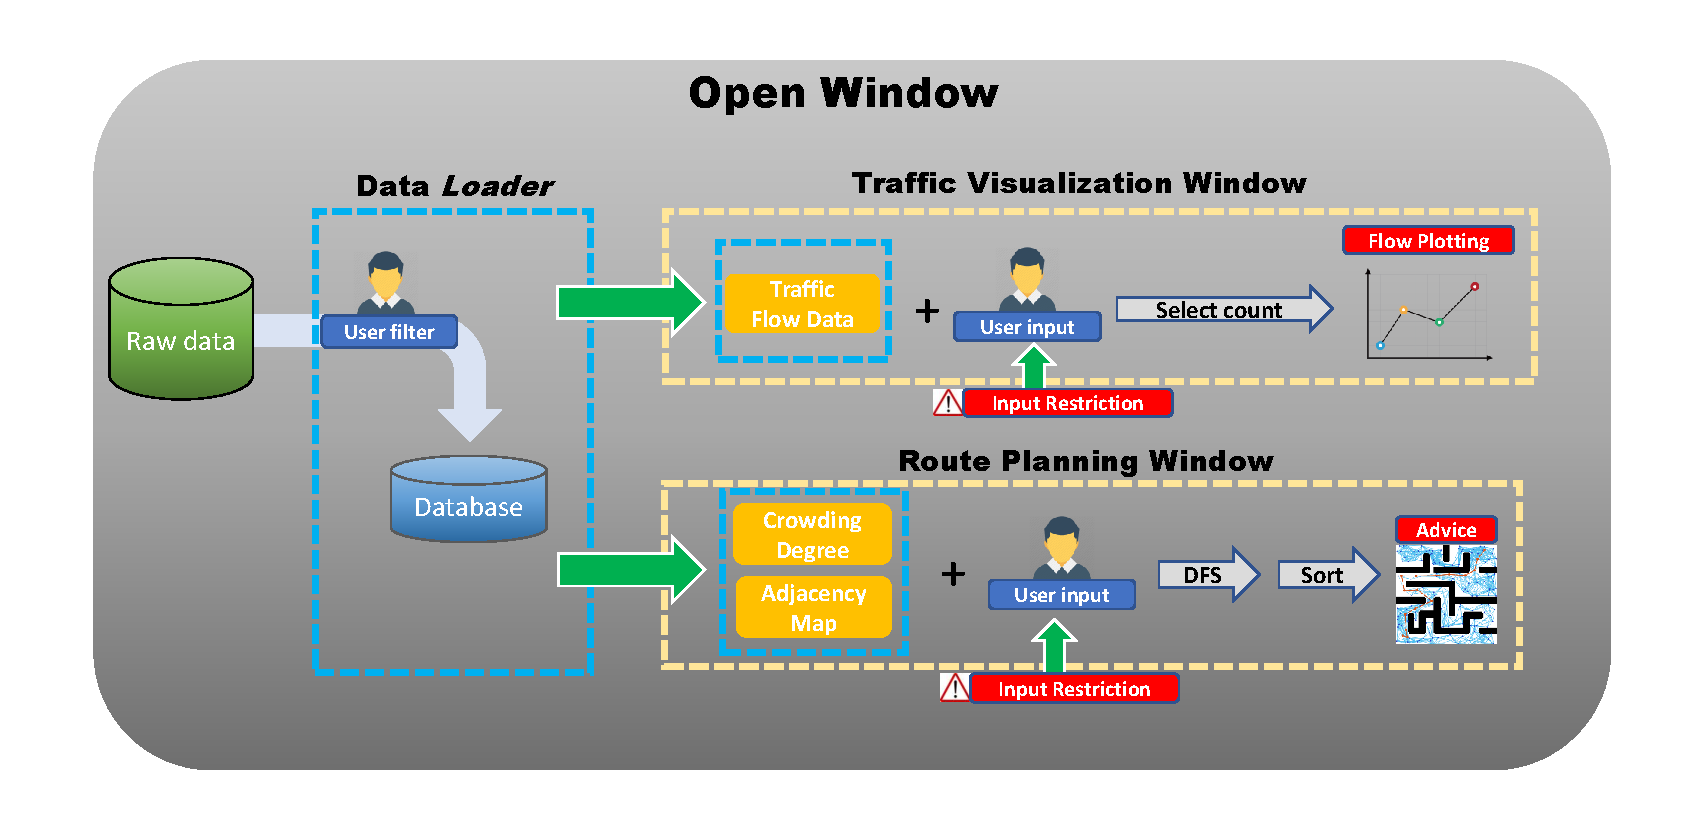
\includegraphics[scale=0.3]{pic_data/cs241_structure.pdf}}
    \caption{Ui Structure}
    \end{figure}



  \subsubsection{Route planning}
  Route planning window is created to make route advice for users. The users can input their departure station number and 
  their destination station number and get a optimzed travelling route. I use DFS to make a search in the adjancencu map,
  and save all the possible route. For each possible, a score is calculated based on the following equation:

  \begin{equation}
    Score[i] = w_l{L[i]} + w_a{A[i]} + w_c{C[i]} (i=1,2, ... n)
  \end{equation}

  where $L[i], A[i], C[i]$ are the length, station changing numbers and the crowding degree of the 
  ith possible route. This is base on the everday feeling: the longer way and more station changing 
  will make the journey time consuming, the more crowding station is always not preferred.
  $w_l,w_a,w_c$are the coefficeints of the three factors, which represent the important of each 
  factor. I set them to  0.5, 0.3, 0.2respectively. The lower the score, the more preferred the route.

  It should be noted that the calculation of length is based on the simple assumption that(L(i, j)
  represents the distance between station i and station j):

  \begin{equation}
    L(i, j) > L(i^{'}, j^{'}) (|i - j| > |i^{'} - j^{'}|)    
  \end{equation}
   For example, the distance between station 1 and station 10 is larger than that between station 1 and 3 at most time.
   So the length of the route can be computed as($n_i$ is the station number in route i, L[i][j] is the number of the j-th station 
   in route i):

  \begin{equation}
    L[i] = \sum_{1}^{j = n_i - 1}{\bigg{|}L[i][j+1] - L[i][j]\bigg{|}}
  \end{equation}

  The crowding degree is calculated simply based on the prior data in the database, and $C[i] = n_i$.After computing all of the 
  scores, I sorted them and select top-2 which have a lower scrore: route1 and route2. route2 will be deleted if:
\begin{equation}
  2S(route1)  < S(route2)
\end{equation}

  \subsubsection{Visualization of metro traffic flow}
  This part is designed to make the data more touchable for the users.In this window.  users can set the stationID, time scope and
  time step to get a line chart of the in-out flow of the selected station. The interpolatory spline is used if the number of sample
  is less than 15 to make the curve more smooth. The passenger flow here are defined as the total number of people entered or leaved 
  the certain station in the time scope. Some discussions about it can be referred to in the section 4.
  In this part I also implemented a visualization of the crowding degree of stations in 
  different lines to make the users have a general view of the 
  metro traffic overcrowding.


\subsection{Polished Ui design}
   In order to make the users have a better experience and at the same time
  integrating into it the characteristics of Hangzhou, I made a polishment of the user interface
   especially on background of windows and the widgets' outlook. I 
   selected some of the typical city elements of Hangzhou including the West Lake the and
   morden city's night view. It actually took me a lot of time to make the layout and
   color of widgets like buttons, text and input boxes matching the background.
   More designs can be seen in the Result part.

\section{Results}
In this part, I will show some images from the user's angle of this Ui(from Figure 2 to 5).
Some time-consumption(TIME CMD) data will also be presented in this part(Table 1).

\begin{figure}
  \centerline{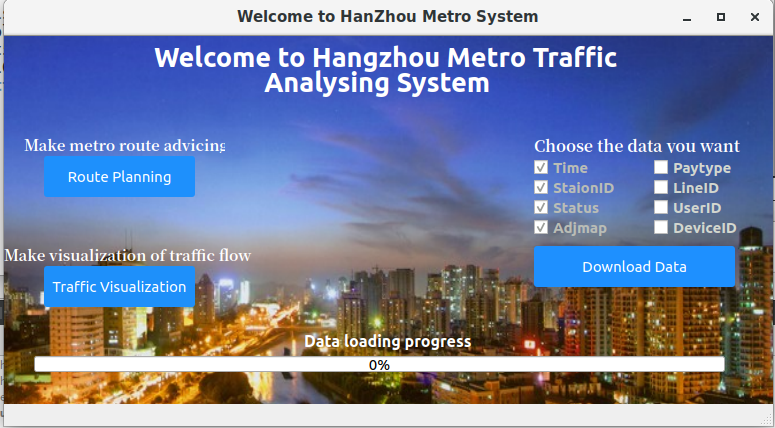
\includegraphics[scale=0.3]{pic_data/openwindow.PNG}}
  \caption{Ui design of openwindow:Night view of Hangzhou}
  \end{figure}

  \begin{figure}
    \centerline{\includegraphics[scale=0.3]{pic_data/routeadv.PNG}}
    \caption{Ui design of data visualization window: Hangzhou traffic}
  \end{figure}

    \begin{figure}
      \centerline{\includegraphics[scale=0.3]{pic_data/viswindow.PNG}}
      \caption{Ui design of route planning window: Beautiful West Lake}

      \end{figure}

      \begin{figure}
        \centerline{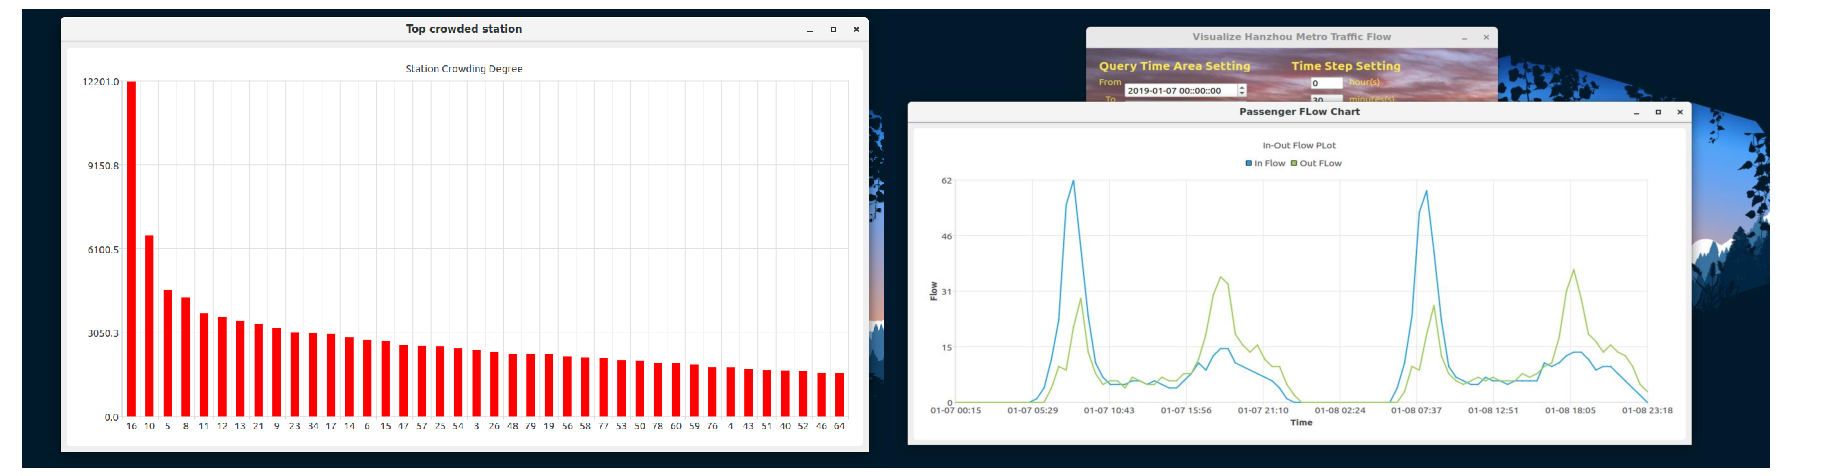
\includegraphics[scale=0.3]{pic_data/plotd.pdf}}
        \caption{Data visualization}
        \end{figure}

        \begin{table}
          \centering
        \caption{\textbf{TIME CMD}}
        \label{table}
        \setlength{\tabcolsep}{3pt}
        \begin{tabular}{|p{125pt}|p{125pt}|}
          \hline
        Function & Average Time Consumption \\
        
        \hline
        Data loading(1 file) & 1007 ms \\
        Data inserting(All) &  3.5 min \\ 
        Route planning &  19 ms\\
        Flow visualization &  1042 ms\\
        
        
        \hline
        \end{tabular}
        \label{tab1}
        \end{table}

\section{Discussion}
   



\end{document}
